\section{Bounding the asynchronous rumour spreading time}
\label{AsyncUpperBoundSection}

In this section we define an algorithm for rumour spreading on a dynamic network, and prove a bound from \cite{asyncPaper} on the associated spreading time that holds with high probability. We then investigate how useful this bound is in practice by applying it to a selection of simple dynamic networks, and comparing the results with simulated spreading times. 

\subsection{Introducing the Rumour Spreading Model}
Now we are ready to define our first asynchronous algorithm for rumour spreading on a given dynamic network.

\begin{definition}
	Push-Pull Asynchronous Rumour Spreading Algorithm 
\end{definition}
\label{NodeCentricAsyncAlgorithm}

\noindent
An asynchronous rumour spreads on a given dynamic network $\mathcal{G} = (G_t)_{t\in \mathbb{N}}$ in rounds. Initially a single node is aware of the rumour. In round $t$, each node is associated with a unit rate exponential clock. When the clock of an informed node $u$ ticks, another node $v$ is selected uniformly at random from the set of neighbouring nodes in $G_t$. $u$ then instantaneously informs $v$ of the rumour if $v$ was not already informed (PUSH). Similarly, when the clock of an uniformed node ticks, it chooses one of its neighbours uniformly at random, and becomes aware of the rumour if the chosen neighbour is an informed node. Each round lasts for a unit time. % TODO: Change final line

% TODO: DEFINE 'UNIT RATE CLOCK' and how it functions (eg what happens after infomed a node)

% TODO: What happens in the case where the node has no neighbours?

% TODO: Implications of this model

\subsection{Proof of the bound}

We follow a proof from \cite{asyncPaper}, explaining steps in greater detail than in the original paper.

First we prove a lemma about how long it takes for the number of nodes aware of the rumour to increase by a multiplicative factor. 

\begin{lemma} \label{AsyncIncreaseLemma}
	Let $\mathcal{G}=(G_t)_{t \in \mathbb{N}}$ be an $n$-node dynamic network. At $t=0$ a single node is aware of rumour which spreads according to algorithm \ref{NodeCentricAsyncAlgorithm}. Choose an arbitrary time $\tau \in [0, \infty)$. We denote the set of informed nodes at this time $I_\tau$, and set uninformed nodes $U_\tau$.
	\noindent
	Define 
	
	$$
	\Delta(\alpha) = \min \left\{t: \sum_{k=0}^t \Phi(G_{\ceil{\tau}+k})\rho(G_{\ceil{\tau}+k}) \geq 2 \alpha \right\}
	$$

	\noindent
	Let $\tau'$ denote the earliest time when $|I_t|$ increases by $\frac{m(\tau)}{2}$, where $m(\tau) := \min\{|I_\tau|, |U_\tau|\}$, i.e,

	$$
		\tau' = \min\left\{\gamma : |I_{\gamma}| \geq |I_\tau| + \frac{m(\tau)}{2}\right\}
	$$
	\noindent
	Then, 
	$$
		\mathbb{P}(\tau' - \tau \geq \Delta(\alpha) + 2) \leq e^{-c\alpha m(\tau)}
	$$
	\noindent
	where $c = \frac{1}{2} - \frac{1}{e}$
\end{lemma}

% TODO: Exposition about interpretation here, dependeces (ie what is m(t) dependent on? et)

At first sight, it may be difficult to identify the relationship that this lemma expresses, so we first explore the implications of the result, before moving to the proof.

When less than half of the nodes are aware of the rumour, we can interpret $\tau'$ as the first time at which the number of informed nodes increases by a half, compared to number of informed nodes at time $\tau$. In this case $|I_{\tau'}| \approxeq \frac{3}{2} |I_\tau|$. When more than half of the nodes are informed, $\tau'$ is the first time at which the set of uniformed nodes shrinks in size by a half, i.e $|U_{\tau'}| \approxeq \frac{|U_\tau|}{2}$. Thus, the random quantity of interest $\tau'-\tau$ is the amount of time it takes for the number of informed nodes to expand by a multiplicative factor, from time $\tau$. 

In the lemma we are interested in the event that this time exceeds $\Delta(\alpha) + 2$. 
The  $+2$ arises from technicalities in the proof, however the $\Delta(\alpha)$ term reveals a relationship between to the rate at which the set of informed nodes expands, and the connectivity of the dynamic network. % TODO: Change the end of this sentance?
Suppose we fix $\alpha$ and $\tau$. From the definition of $\Delta(\alpha)$ we see that the greater the conductance and diligence metrics of the static topologies in the time steps immediately after $\tau$, the smaller the value of $\Delta(\alpha)$ becomes, since the summation will exceed $2\alpha$ in fewer terms. Thus, we see that well-connected topologies will yield smaller values of $\Delta(\alpha)$. Returning to the probability bound, we see that the bounding term $e^{-c\alpha m(\tau)}$ is independent of the topologies after $\tau$. Thus the bound tells us that the better the connectivity, the shorter the time it takes for the rumour to spread by a multiplicative factor (under the same probability). % TODO: Change bracketed bit to make more sense or remove
This supports our intuitive expectation that rumour spreading using algorithm \ref{NodeCentricAsyncAlgorithm} is faster in well-connected dynamic networks. % TODO: SHOULD WE EXPECT THIS? HIGHER CONNETIVITY => HIGER DEGREE => LOWER RATE OF TRANSMISSION BETWEEN INDIVIUDAL PAIRS OF NODES.

% TODO: Sanity check on bound by varying alpha: larger alpha => larger delta(alpha) => stronger bound below => tighter proabilitstic bound e^stuff


\begin{proof}
	Fix a time $\gamma \in [\tau, \tau')$. 
	We consider the set of edges $E(I_\gamma, U_\gamma)$ between the informed and uninformed sets of nodes at time $\gamma$. 
	Let $\{u, v\} \in E(I_\gamma, U_\gamma)$. By the thinning property of Poisson processes, node $u$ pushes the rumour to $v$ according to a Poisson process of rate $\frac{1}{d_u(\gamma)}$. Similarly, node $v$ pulls the rumour from $u$ according to a Poisson process of rate $\frac{1}{d_v(\gamma)}$. % TODO: Why does this hold? - exposition
	Thus, by the superposition property of Poisson processes, the time until the first uniformed node is made aware of the rumour has an exponential distribution of rate % TODO: Why does this hold - or minimum of exponentials
	$$
		\lambda(\gamma) = \sum_{\{u, v\} \in E(I_\gamma, U_\gamma)} \frac{1}{d_u(\gamma)} + \frac{1}{d_v(\gamma)}
	$$
	% TODO: DIAGRAM HERE LABELLED WITH RATES
	Let $S = I_\gamma$ if $\text{vol}(I_\gamma) \leq \text{vol}(U_\gamma)$, otherwise let $S = U_\gamma$. Then,

	%TODO: Justify all steps
	\begin{align*}
		\lambda(\gamma) &= \sum_{\{u', v'\} \in E(I_\gamma, U_\gamma)} \left\{ \frac{1}{d_{u'}(\gamma)} + \frac{1}{d_{v'}(\gamma)} \right\}\\
		& \geq \sum_{\{u', v'\} \in E(I_\gamma, U_\gamma)}  \max \left\{ \frac{1}{d_{u'}(\gamma)},\frac{1}{d_{v'}(\gamma)} \right\} \\ 
		% TODO: Justify above
		& \geq \sum_{\{u', v'\} \in E(I_\gamma, U_\gamma)} \min_{\{u, v\} \in E(I_\gamma, U_\gamma) } \left\{ \max \left\{ \frac{1}{d_u(\gamma)},\frac{1}{d_v(\gamma)} \right\} \right\} & \\ 
		& = \min_{\{u, v\} \in E(I_\gamma, U_\gamma) } 
		\left\{ \max \left\{ \frac{1}{d_u(\gamma)},\frac{1}{d_v(\gamma)} \right\} \right\} |E(I_\gamma, U_\gamma)| \\
		%TODO: Mention degrees indexed by time above?
		& = \rho(S) \frac{|S|}{\text{vol}(S)} |E(I_\gamma, U_\gamma)| \\
		& = \rho(S) |S| \frac{|E(I_\gamma, U_\gamma)|}{ 
			\min\{\text{vol}(I_\gamma), \text{vol}(U_\gamma)\}
		} \\
		& \geq \rho(G_\gamma)\Phi(G_\gamma)|S| \\ 
		% TODO: Since We instantiate at specific sets
		& \\
		& \geq \rho(G_\gamma)\Phi(G_\gamma) \min\{|I_\gamma|, |U_\gamma|\} \\
		& \text{since } S = I_\gamma \text { or } U_\gamma \\
		& \\
		& = \rho(G_\gamma)\Phi(G_\gamma) m(\gamma) \\
		& \text{by the definition of } m(\gamma)
	\end{align*}
	% TODO: Brief exposition here
	We now procceed to prove the following claim, by performing case analysis on $m(\gamma)$

	\textbf{Claim.} $m(\gamma) \geq \frac{m(\tau)}{2}$. % Inutive explanation

	\textbf{Case 1.} Suppose $m(\gamma) = |I_\gamma|$

	\noindent
	Once a node is aware of the rumour it never becomes uninformed. Hence, as $\tau \leq \gamma$, at time $\gamma$ there are at least $|I_\tau|$ informed nodes, thus 
	$$
	|I_\gamma| \geq |I_\tau| \geq \frac{|I_\tau|}{2} \geq \frac{m(\tau)}{2}
	$$
	so the claim holds in this case.

	\textbf{Case 2.} Suppose instead that $m(\gamma) = |U_\gamma|$

	\noindent
	By the defintion of $\tau'$, since $\gamma < \tau'$ we have that $|I_{\gamma}| < |I_\tau| + \frac{m(\tau)}{2}$.

	Since $|I_t| + |U_t| = n$ for all times $t$, note that
	$$
		|I_{\gamma}| < |I_\tau| + \frac{m(\tau)}{2} 
		\iff
		n - |U_{\gamma}| < n - |U_\tau| + \frac{m(\tau)}{2} 
		\iff
		|U_\gamma| > |U_\tau| - \frac{m(\tau)}{2}
	$$
	Thus we have that
	\begin{align*}
		|U_\gamma| & > |U_\tau| - \frac{m(\tau)}{2} & \text{since }\gamma < \tau' \\
		& \geq |U_\tau| - \frac{|U_\tau|}{2} & \text{since } m(\tau) \leq |U_\tau| \\
		& = \frac{|U_\tau|}{2} \\
	\end{align*}
	Thus the claim holds in this case also.
	
	\noindent
	By applying the claim to the final inequality in the previous chain of inequalities we get that
	\begin{equation} \label{eq:RateBound}
		\lambda(\gamma) \geq \rho(G_\gamma)\Phi(G_\gamma)\frac{m(\tau)}{2}
	\end{equation}

	So far we have bounded the rate at which uninformed nodes are made aware of the rumour at time $\gamma$. Since the rate of transmission is a function of $\gamma$ we define an inhomogeneous Poisson process $\{N(\gamma), \gamma \geq \tau\}$ with rate function $\lambda(\gamma)$. % TODO: Is this a poisson proccess? Independent increments, rate function defined by realisation but still has independet increments, step talk about step function.
	Intuitively, $N(\gamma)$ counts the number of newly informed nodes in the interval $[\tau,\gamma)$. %TODO: Change last sentance - exactly the same as paper


	By [CITE INHOMOGENOUS THEROEM], $N(\tau + \Delta(\alpha) + 2)$ has a Poission distribution with rate $\Lambda(\tau + \Delta(\alpha) + 2)$, where
	\begin{align*}
		\Lambda(\tau + \Delta(\alpha) + 2) &= \int_\tau^{\tau + \Delta(\alpha) + 2} \lambda(\gamma) d\gamma \\
		& \geq \int_{\ceil\tau}^{{\ceil\tau} + \Delta(\alpha) + 1} \lambda(\gamma) d\gamma \\
		& \text{since } \lambda(\gamma) \geq 0 \text{ as it is a rate function}\\
		& \\
		& = \sum_{k=0}^{\Delta(\alpha)} \int_{\ceil\tau + k}^{{\ceil\tau} + k + 1} \lambda(\gamma) d\gamma \\
		& \text{by splitting the integral into unit length intervals } \\
		& \\
		& \geq \sum_{k=0}^{\Delta(\alpha)} \int_{\ceil\tau + k}^{{\ceil\tau} + k + 1} \rho(G_\gamma)\Phi(G_\gamma)\frac{m(\tau)}{2} d\gamma \\
		& \text{by applying Inequality } \ref{eq:RateBound} \\
		& \\
		& = \sum_{k=0}^{\Delta(\alpha)} \rho(G_{\ceil\tau + k})\Phi(G_{\ceil\tau + k})\frac{m(\tau)}{2} \\
		& \text{since } G_\gamma = G_{\floor\gamma} \\
		& \\
		& \geq 2\alpha\frac{m(\tau)}{2} \\
		& \text{by the definition of } \Delta(\alpha) \\
		& \\
		& = \alpha m(\tau)
	\end{align*}
	Let $X$ be a random variable with a $\text{Poisson}(\alpha m(\tau))$ distribution. 
	By the previous chain of inequalities we have that $X$ is stochastically dominated by $N(\tau + \Delta(\alpha) + 2)$. % TODO: Talk about stochastic domination
	Note that
	$$
		\tau' - \tau \geq \Delta(\alpha) + 2 \iff 
		\tau' \geq \tau + \Delta(\alpha) + 2 \implies 
		N(\tau + \Delta(\alpha) + 2) \leq \frac{m(\tau)}{2}
	$$
	where the final implication holds since by the definition of $\tau'$, if $\tau' \geq \tau + \Delta(\alpha) + 2$ then the number of new nodes informed of the the rumour between time $\tau$ and $\tau + \Delta(\alpha) + 2$ must be less than or equal to $\frac{m(\tau)}{2}$. Hence we have that
	\begin{align*}
		\mathbb{P}(\tau' - \tau \geq \Delta(\alpha) + 2) & 
		\leq \mathbb{P}\left(N(\tau + \Delta(\alpha) + 2) \leq \frac{m(\tau)}{2}\right) \\
		& \leq \mathbb{P}\left(X \leq \frac{m(\tau)}{2}\right) \\
		& \text{since } X \text{ is stochastically dominated by } N(\tau + \Delta(\alpha) + 2) \\
		& \\
		& \leq \mathbb{P}\left(X \leq \frac{\alpha m(\tau)}{2}\right) \\
		& \text{since } \alpha \geq 1 \\ % TODO: Check this assumption
	\end{align*}
	To finish the proof we prove the following claim

	\noindent
	\textbf{Claim.} For a Poisson($r$) distributed random random variable $Y$, 
	$$
		\mathbb{P}(Y \leq \frac{r}{2}) \leq e^{-cr}
	$$
	where $c$ is the constant defined in the statement of Lemma \ref{AsyncIncreaseLemma}.

	\noindent
	\textit{Proof of Claim}

	\noindent
	From the definition of the density function of Poisson random variables we have that 
	\begin{align*}
		\mathbb{P}(Y \leq \frac{r}{2}) & = e^{-r} \sum_{j=0}^\frac{r}{2} \frac{r^j}{j!} \\ % TODO: Assumes r/2 is integer? - add floor to upper bond of sum
		& = e^{-r} \sum_{j=0}^\frac{r}{2} \frac{2^j(\frac{r}{2})^j}{j!} \\
		& \leq e^{-r} \sum_{j=0}^\frac{r}{2} \frac{2^\frac{r}{2}(\frac{r}{2})^j}{j!} \\
		& \leq e^{-r} e^\frac{r \log 2}{2} \sum_{j=0}^\frac{r}{2} \frac{(\frac{r}{2})^j}{j!} \\
		& \leq e^{-r} e^\frac{r \log 2}{2} e^\frac{r}{2} \\
		& = e^{-r(\frac{1}{2} - \frac{\log2}{2})} \\ % TODO: Weaken constant?
	\end{align*}
	thus the claim is proved. Since $X \sim \text{Poisson}(\alpha m(\tau))$ we get that
	\begin{align*}
		\mathbb{P}(\tau' - \tau \geq \Delta(\alpha) + 2) \leq \mathbb{P}(X \leq \frac{\alpha m(\tau)}{2}) \leq e^{-c \alpha m(\tau)}
	\end{align*}	
\end{proof}

Now we iteratively apply Lemma \ref{AsyncIncreaseLemma} to derive the following Theorem.

\begin{theorem}\label{theorem:AsyncUpperBound}
	\ModelIntro Then, with high probability, the rumour will have spread to all the nodes of $\mathcal{G}$ in time at most

	$$
		\min \left\{t : \sum_{k=0}^t \Phi(G_k)\rho(G_k) \geq C \log n \right\} 
	$$

	\noindent
	for a sufficiently large $C$
\end{theorem}

\begin{proof}
	We analyse the spread time in two phases. 

	% TODO: Add a of phase and intervals here, maybe plot m(t)

	\textbf{First Phase.} The first phase starts at time $t=0$ and ends at the first time when the number of informed nodes reaches $\frac{n}{2}$, which we denote $t_\text{half}$. We divide the phase into intervals $[\tau_i, \tau_{i+1}]$ where $\tau_0 = 0$ and $\tau_{i+1}$ is the first time the number of informed nodes increases by $\frac{m(\tau_i)}{2}$. 
	% TODO: MENTION FINAL INTERVAL MAY END AFTER t_\text{half}
	Using the notation from Lemma \ref{AsyncIncreaseLemma}, we have that $\tau_{i+1} = \tau_i'$. 
	
	Note that for all times $\tau < t_\text{half}$, the number of informed nodes is less than $\frac{n}{2}$, so $m(\tau) = |I_\tau|$. Thus, by the following induction at time $\tau_i < t_\text{half}$ there are at least $(\frac{3}{2})^i$ informed nodes.

	\underline{Base Case.}
	By algorithm \ref{NodeCentricAsyncAlgorithm} the rumour spreading starts at time 0 with a single node aware of the rumour. Thus $|I_{\tau_0}| = 1 = (\frac{3}{2})^0$

	\underline{Inductive Case.} 
	Assume that $\tau_i \geq (\frac{3}{2})^i$.
	From the definition of $\tau_i'$, we have that 
	\begin{align*}
		\tau_{i+1} &= \tau_i' \\
		&= \min\left\{\gamma : |I_{\gamma}| \geq |I_{\tau_i}| + \frac{m(\tau_i)}{2}\right\} \\
		&= \min\left\{\gamma : |I_{\gamma}| \geq |I_{\tau_i}| + \frac{|I_{\tau_i}|}{2}\right\} & \text{since } m(\tau_i) = |I_{\tau _i}| \text{ in this phase} \\ 
		&= \min\left\{\gamma : |I_{\gamma}| \geq \frac{3}{2}|I_{\tau_i}|\right\} 
	\end{align*}
	Thus $|I_{\tau_{i+1}}| \geq \frac{3}{2}|I_{\tau_i}| \geq \frac{3}{2}(\frac{3}{2})^i = (\frac{3}{2})^{i+1}$ by the induction hypothesis. 
	
	Let $K$ be the random variable for the index of the final interval in the phase, i.e the interval where $\tau_K < t_\text{half}$ and $\tau_{K+1} \geq t_\text{half}$.
	% TODO: TIMELINE FIGURE HERE
	Let $N = \ceil{\log_\frac{3}{2}\frac{n}{2}}$.  Since $|I_{\tau_i}| \geq (\frac{3}{2})^i$, we have that $|I_{\tau_N}| \geq (\frac{3}{2})^N \geq \frac{n}{2}$. Thus, $K < N$ otherwise the number of informed nodes at time $\tau_K$ would be greater than or equal to $\frac{n}{2}$, so $\tau_K$ would be at least $t_\text{half}$ which contradicts the definition of $K$.

	Let $\alpha_i = \ceil{\frac{c \log n}{c_0 (3/2)^i}}$. % TODO: Are c_0 and C defined? 
	By Lemma \ref{AsyncIncreaseLemma}, $\Delta(\alpha_i) + 2$ is an upper bound for the length of the interval $[\tau_i, \tau_{i+1}]$ 
	with probability at least $1 - e^{-c_0\alpha_i m(\tau_i)}$. %TODO: RESTRICT to i \leq K
	Since $m(\tau_i) = |I_{\tau_i}| \geq (\frac{3}{2})^i$, this probability is greater than $1 - e^{-c_0\alpha_i (\frac{3}{2})^i} \geq 1 - e^{-c \log n}$, by the definition of $\alpha_i$. By the union bound over all $K$ intervals of the phase,
	\begin{align*}
		& \mathbb{P}(\text{Any interval has length at least } \Delta(\alpha_i) + 2) \\
		&= \mathbb{P}(\bigcup_{i=0}^K \{\tau_{i+1} - \tau_i \geq \Delta(\alpha_i) + 2\}) \\
		&\leq \sum_{i=0}^K \mathbb{P}(\tau_{i+1} - \tau_i \geq \Delta(\alpha_i) + 2) \\
		&\leq \sum_{i=0}^K e^{-c \log n} \\
		&\leq \sum_{i=0}^N e^{-c \log n} 
		%% TODO: PUT IN REASONING& \text{since } K < N 
		\\
		&= N e^{-c \log n} \\
		&\to 0 \text { as } n \to \infty
	\end{align*}
	Thus with high probability all intervals have length at least $\Delta(\alpha_i) + 2$, hence
	\begin{align*}
		t_\text{half} &\leq \sum_{i=0}^K (\Delta(\alpha_i) + 2) \\
		&\leq \min \{t : blah \geq 2 \sum_{i=0}^K \alpha_i \} \\ % TODO: Justify this step
		&\leq \min \{t : blah \geq 2 \sum_{i=0}^N \alpha_i \} & %TODO: Mention \alpha_i need to be defined up to N
	\end{align*}

	\textbf{Second Phase.} The second phase starts at $t_\text{half}$, when at least $\frac{n}{2}$ nodes have been made aware of the rumour. The phase ends at the first time all nodes are aware of the rumour, which we denote $t_\text{all}$. We again divide up the phase into intervals $[\tau_j, \tau_{j+1}]$, where $\tau_0 = t_\text{half}$ and $\tau_{j+1} = \tau_j'$ as in the first phase.

	Note that since the number of informed nodes is at least $\frac{n}{2}$ during this is phase, the number of uninformed nodes is at most $\frac{n}{2}$. Thus for $\tau > t_\text{half}$, $m(\tau) = |U_\tau|$. Using this fact, we prove $|U_{\tau_j}| \leq n(\frac{1}{2})^{j+1}$ by induction.

	\underline{Base Case.}
	From the definition of $t_\text{half}$, $|I_{\tau_0}| = |I_{t_\text{half}}| \geq \frac{n}{2}$, so $|U_{\tau_0}| \leq \frac{n}{2}$.

	\underline{Inductive Case.} Suppose $|U_{\tau_j}| \leq n(\frac{1}{2})^{j+1}$. Note that since $|I_\tau| + |U_\tau| = n$, we have that $|I_{\gamma}| \geq |I_\tau| + \frac{m(\tau)}{2} \iff |U_\gamma| \leq |U_\tau| - \frac{m(\tau)}{2}$. Hence by the defintion of $\tau_j'$,
	\begin{align*}
		\tau_{j+1} &= \tau_j' \\
		&= \min \{ \gamma : |I_\gamma| \geq |I_{\tau_j}| + \frac{m(\tau_j)}{2}\} \\
		&= \min \{ \gamma : |U_\gamma| \leq |U_{\tau_j}| - \frac{m(\tau_j)}{2}\} \\
		&= \min \{ \gamma : |U_\gamma| \leq |U_{\tau_j}| - \frac{|U_{\tau_j}|}{2}\} & \text{since } m(\tau_j) = |U_{\tau_j}| \text{ in this phase} \\
		&= \min \{ \gamma : |U_\gamma| \leq \frac{1}{2}|U_{\tau_j}|\}
	\end{align*}
	Thus by the induction hypothesis, $|U_{\tau_{j+1}}| \leq \frac{1}{2}|U_{\tau_j}| \leq \frac{1}{2}n(\frac{1}{2})^{j+1} = n(\frac{1}{2})^{j+2}$.

	As in the first phase, let $K$ be the random variable for the index of the final interval in the phase, i.e the interval where $\tau_K < t_\text{all}$ and $\tau_{K+1} \geq t_\text{all}$.

	Let $M = \floor{\log_2 n}$. Since $|U_{\tau_j}| \leq n(\frac{1}{2})^{j+1}$, we have that $|U_{\tau_M}| \leq n(\frac{1}{2})^{M+1} \leq \frac{1}{2}$, thus since the number of informed nodes is an integer, at time $\tau_M$ there are no uninformed nodes left i.e all nodes are informed of the rumour. Hence $K < M$, otherwise at time $\tau_K$ all nodes would be aware of the rumour but we have that $\tau_K < t_\text{all}$ by the definition of $K$.

	Let $\beta_j = \ceil{\frac{c \log n}{c_0 n(1/2)^j}}$. % TODO: Are c_0 and C defined? 
	By Lemma \ref{AsyncIncreaseLemma}, $\Delta(\beta_i) + 2$ is an upper bound for the length of the interval $[\tau_j, \tau_{j+1}]$ 
	with probability at least $1 - e^{-c_0\beta_j m(\tau_j)}$. %TODO: RESTRICT to i \leq K
	Since $m(\tau_j) = |U_{\tau_j}| \leq n(\frac{1}{2})^{j+1}$. % TODO: Need lower bound

\end{proof}

In Theorem \ref{theorem:AsyncUpperBound}, we have successfully generalized standard results about the rumour spreading time to dynamic networks. Indeed, by using Theorem \ref{theorem:AsyncUpperBound} we can recover a standard result about rumour spreading on static networks. If we let $G_t = G$ for all $t$ (i.e. a static network), by Theorem \ref{theorem:AsyncUpperBound} the rumour spreading time $T$ satisfies 
\begin{align*}
	T &= \min \left\{t : \sum_{k=0}^t \Phi(G)\rho(G) \geq C \log n \right\} \\
	&= \min \left\{t : t \Phi(G)\rho(G) \geq C \log n \right\}  \\
	&= \min \left\{t : t \geq \frac{C \log n}{\Phi(G)\rho(G)}\right\}  \\
	&= \mathcal{O}\left(\frac{\log n}{\Phi(G)\rho(G)}\right)
\end{align*}
with high probability. This result is almost identical to a standard result for rumour spreading on static networks.  % TODO: CITE https://people.maths.bris.ac.uk/~maajg/teaching/complexnets/rumours.pdf

% TODO: "however, the real stregth comes from dynamic networks"

% TODO: THIS IS A BIT OF A JUMP, SANITY CHECK?
Theorem \ref{theorem:AsyncUpperBound} also expresses the relationship between the success probability of the bound, and the size of the bound. We recall that the failure probability of the bound is $\mathcal{O}\left(\log(n) e^{-c \log(n)}\right)$, where $c$ is a chosen constant greater than 1. % TODO: Check greater than 1 constraint
We also note that the constant $C$ in Theorem \ref{theorem:AsyncUpperBound} is monotone increasing in $c$. The greater $C$ is, the more terms will be required for the summation to exceed $C \log n$, which will yield a larger bound. 
Thus, the intuitive idea that the greater the success probability of the bound, the larger the bound needs to be, holds. % TODO: Reword this sentance

% BENEFITS

% DRAWBACKS
% CAN'T GET EXPLICIT RESULTS
% - CONSTANT CASE
% NOT DEPENDENT ON ADVERSARIAL REARRANGEMENTS (invariant on relabelling)
% NOT VERY TIGHT IN GENERAL -> HOW CAN WE BE SURE IT GIVES THE CORRECT SCALING? 
% Sequence needs to be known ahead of time - strong restriction

% IN NEXT SECTION WE WILL SEE IT'S ALMOST TIGHT IN SCALING

 
% TODO: TODAY How does diligence affect bound?

\begin{enumerate}
	\item Why diligence useful?
	\item When useful/better than other bounds?
	\item Comparison between absolute and non-absolute  diligence results, when is each useful?
\end{enumerate}

\subsection{Evaluating the bound}

In this section we gauge the quality of the bound by comparing it with simulated spreading times.

\begin{figure}[h]
	\centering
	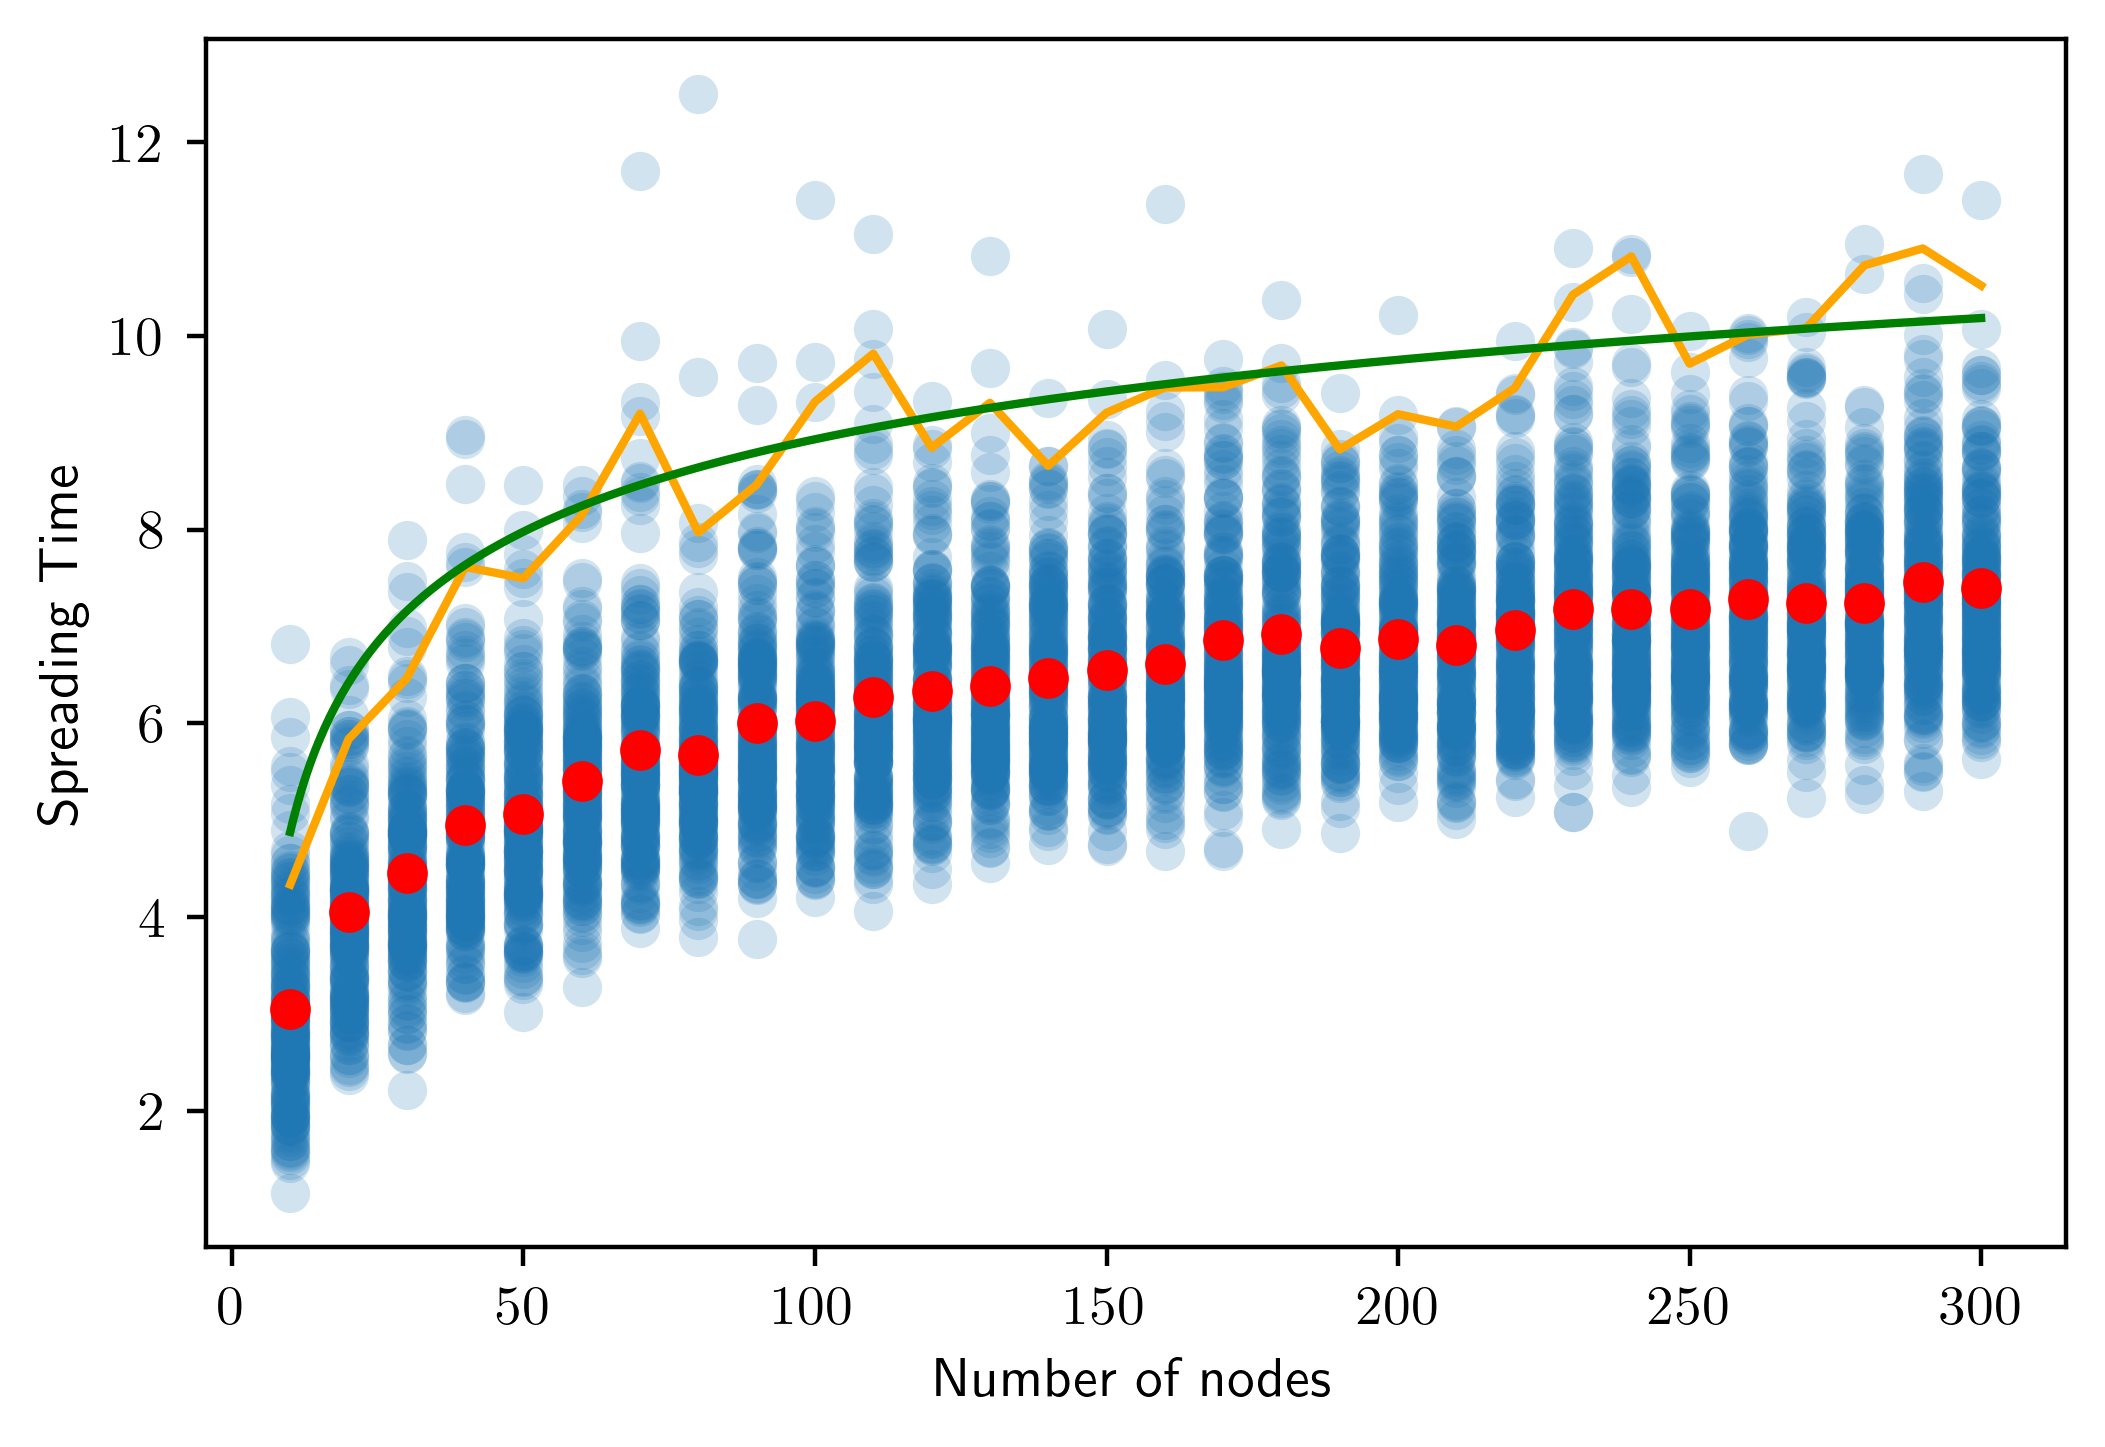
\includegraphics[width=1\textwidth]{./figures/alternating_ring_simulation_results.png}
	\caption{Results of alternating network spreading time simulations}
	\label{fig:alternatingSimResults}
\end{figure}

\begin{figure}[h]
	\centering
	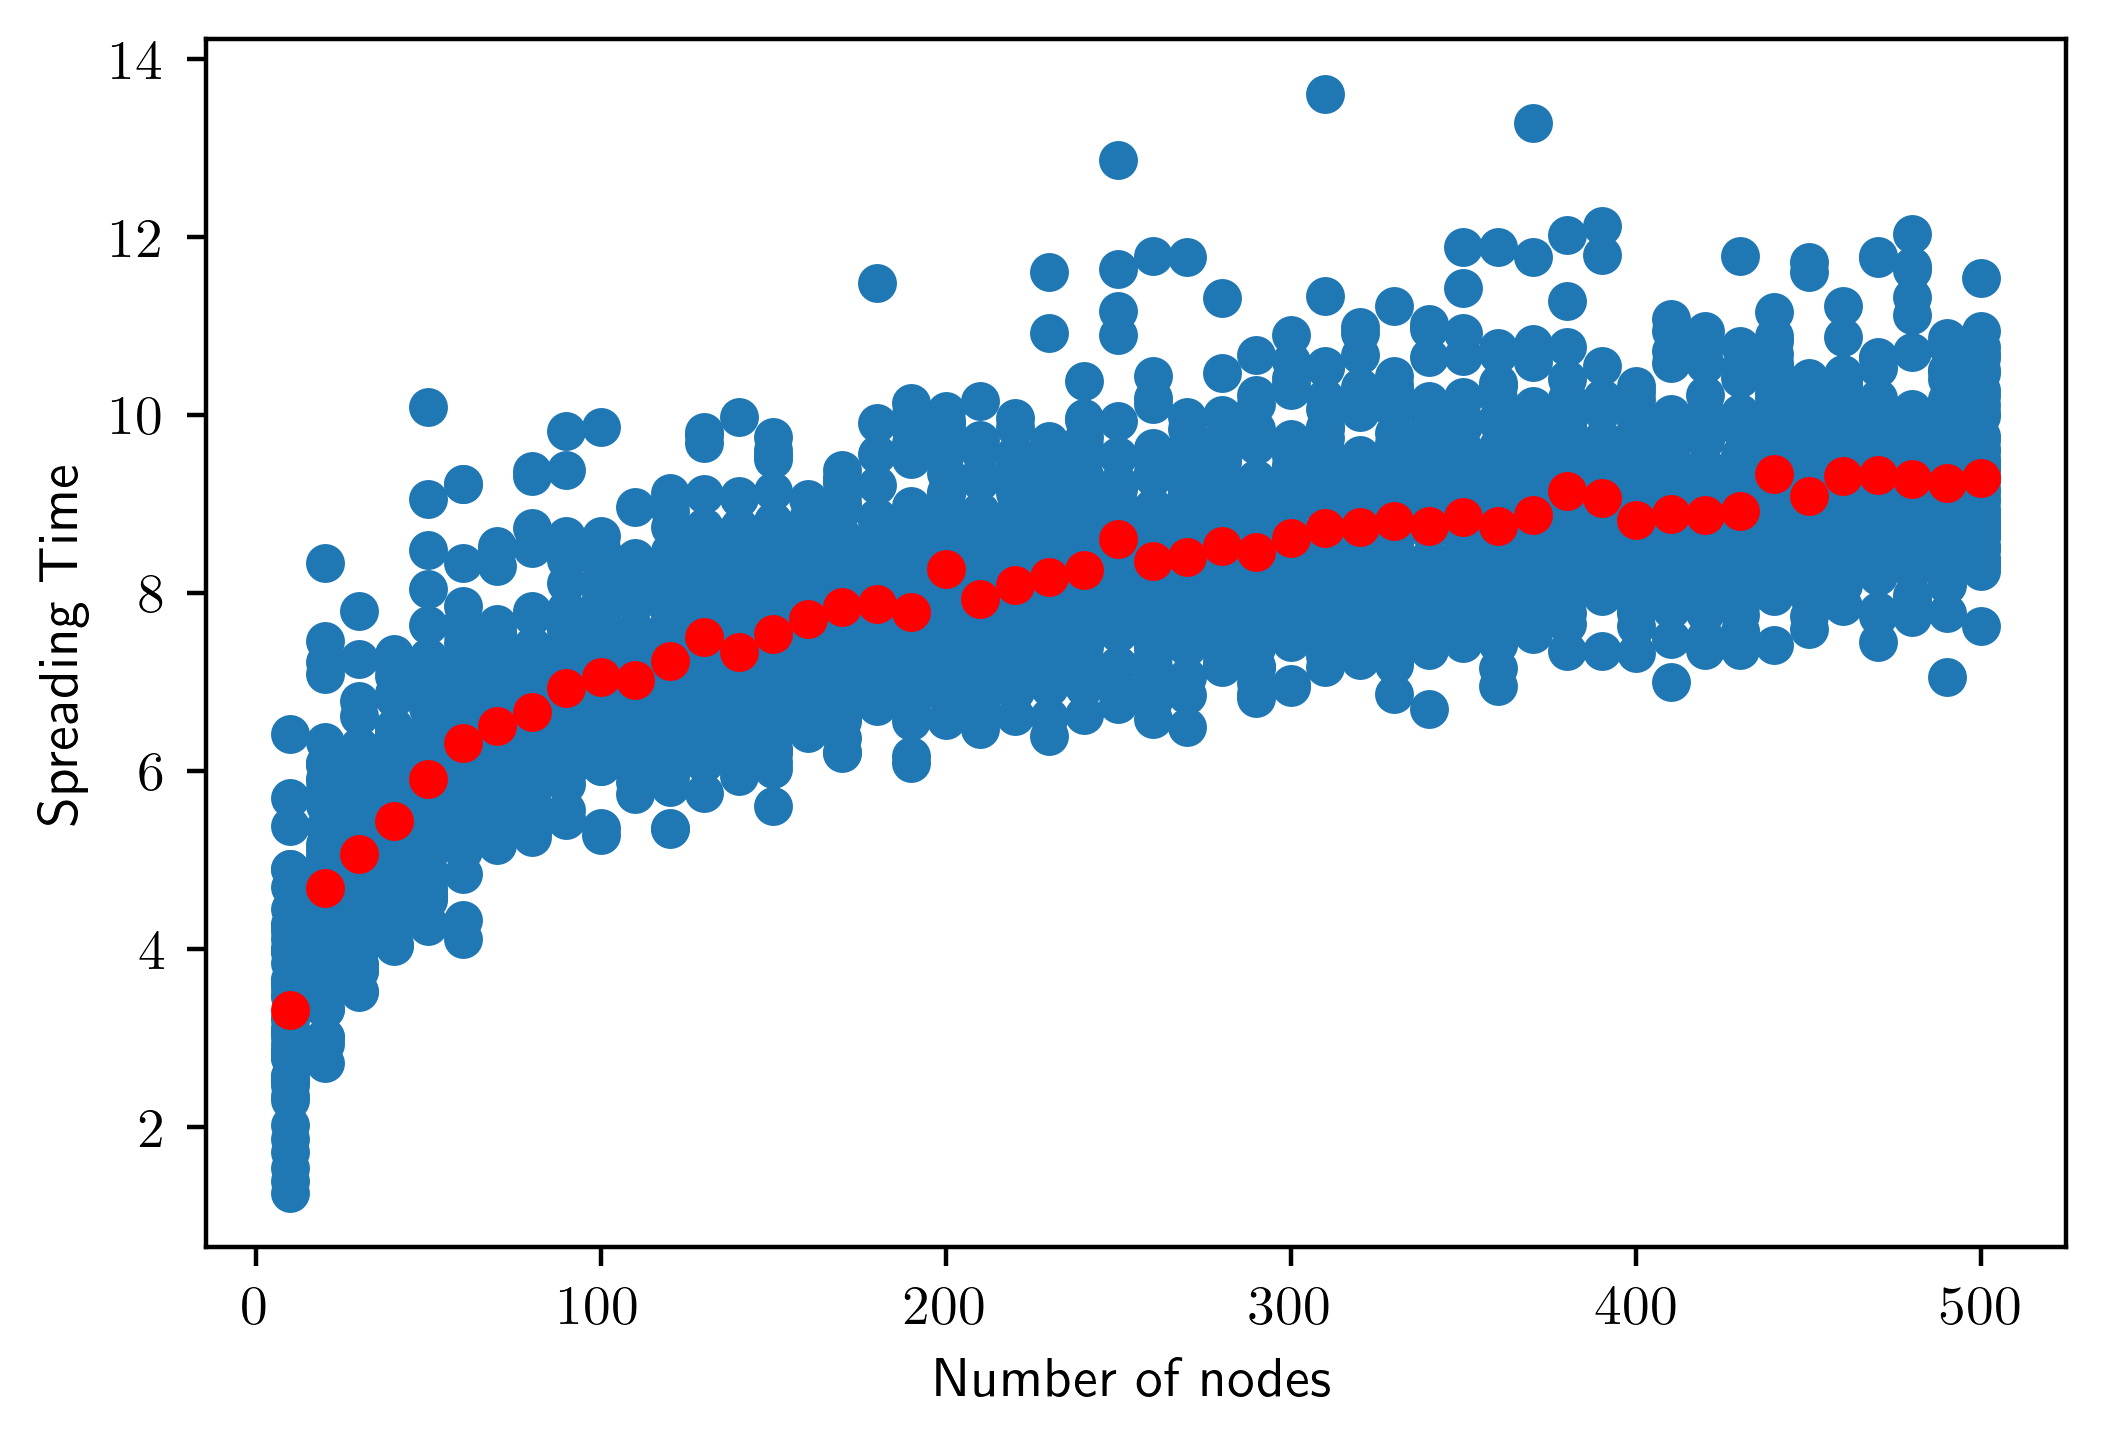
\includegraphics[width=1\textwidth]{./figures/shuffle_ring_simulation_results.png}
	\caption{Results of shuffled ring spreading time simulations}
	\label{fig:shuffleRingSimResults}
\end{figure}

\begin{figure}[h]
	\centering
	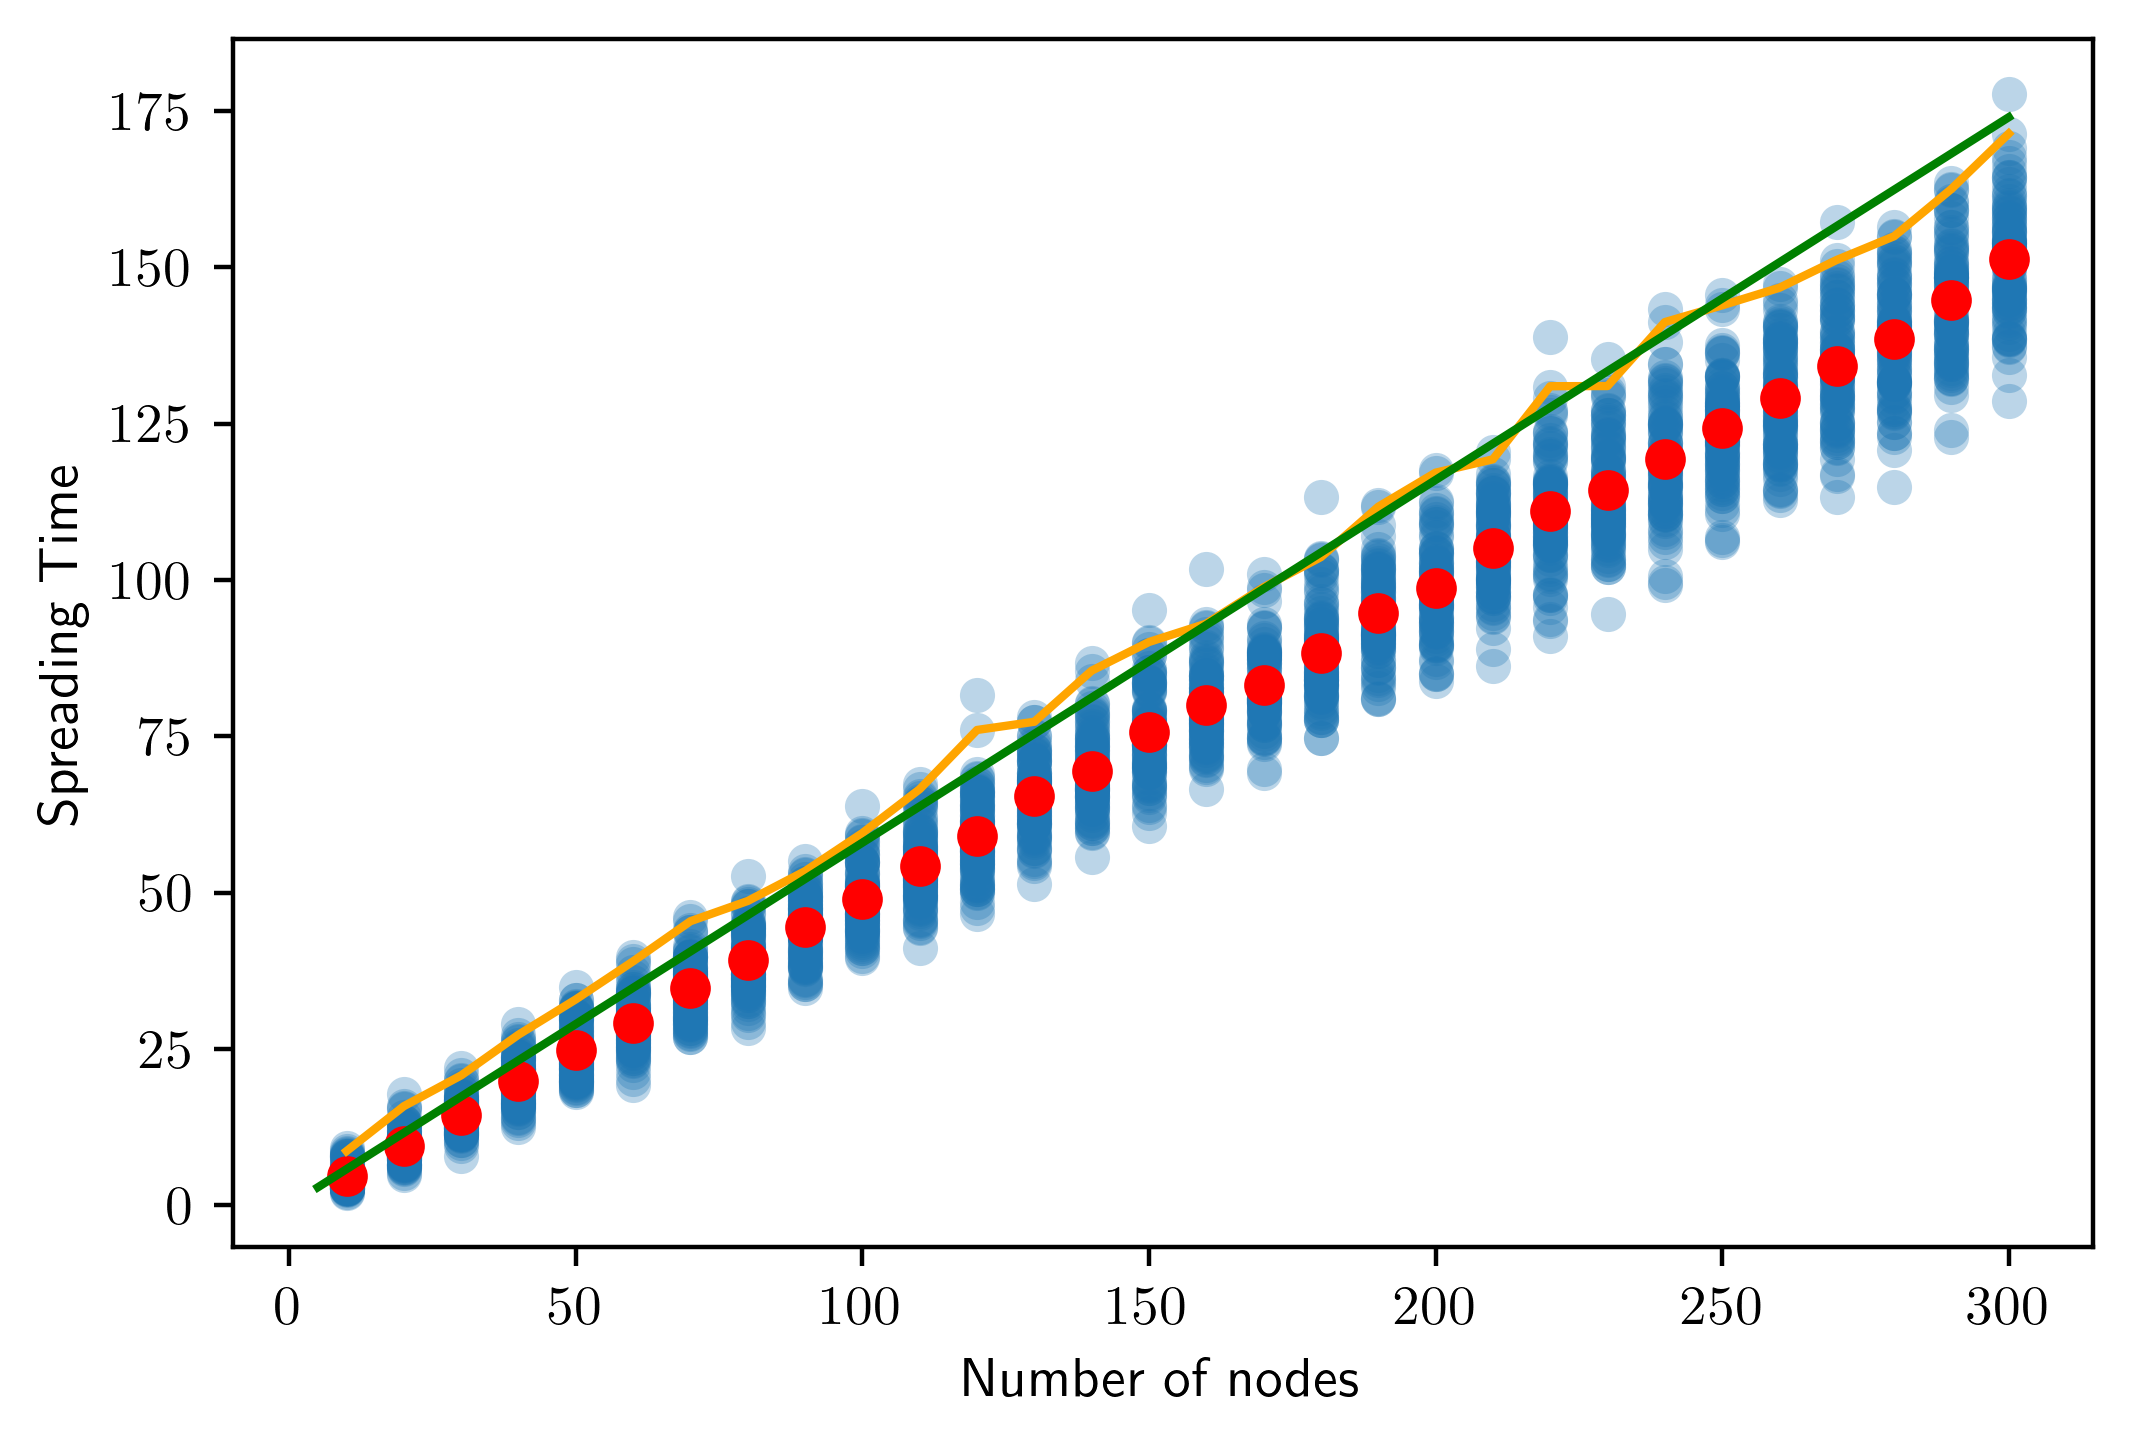
\includegraphics[width=1\textwidth]{./figures/static_ring_simulation_results.png}
	\caption{Results of static ring spreading time simulations}
	\label{fig:staticRingSimResults}
\end{figure}

% TODO: Adversarial not "figting back" but one of the possibilites the bound has to account for